% Staging vs Self-Refine vs Decompose schematic.
%
% Provenance: bound by ci/illustration_lineage.json to the
% Constitutional AI block at main.tex:349-350. The block argues that
% critique-revision is structurally staged constraint satisfaction;
% this schematic makes the contrast with self-refine + decompose
% visually legible.
%
% Composition exploration via gpt-5.4-image-2 returned a narrower
% interpretation (single-flow critique-revision); the deterministic
% redraw widens to the three-protocol comparison the body section
% argues for. The model is a TOOL for visual exploration, not a
% judge of what the comparison should depict.
%
% Claim scope: schematic illustration only; not empirical evidence.
% Token counts cite Table baselines.

\begin{figure}[!htb]
\centering
\resizebox{\linewidth}{!}{%
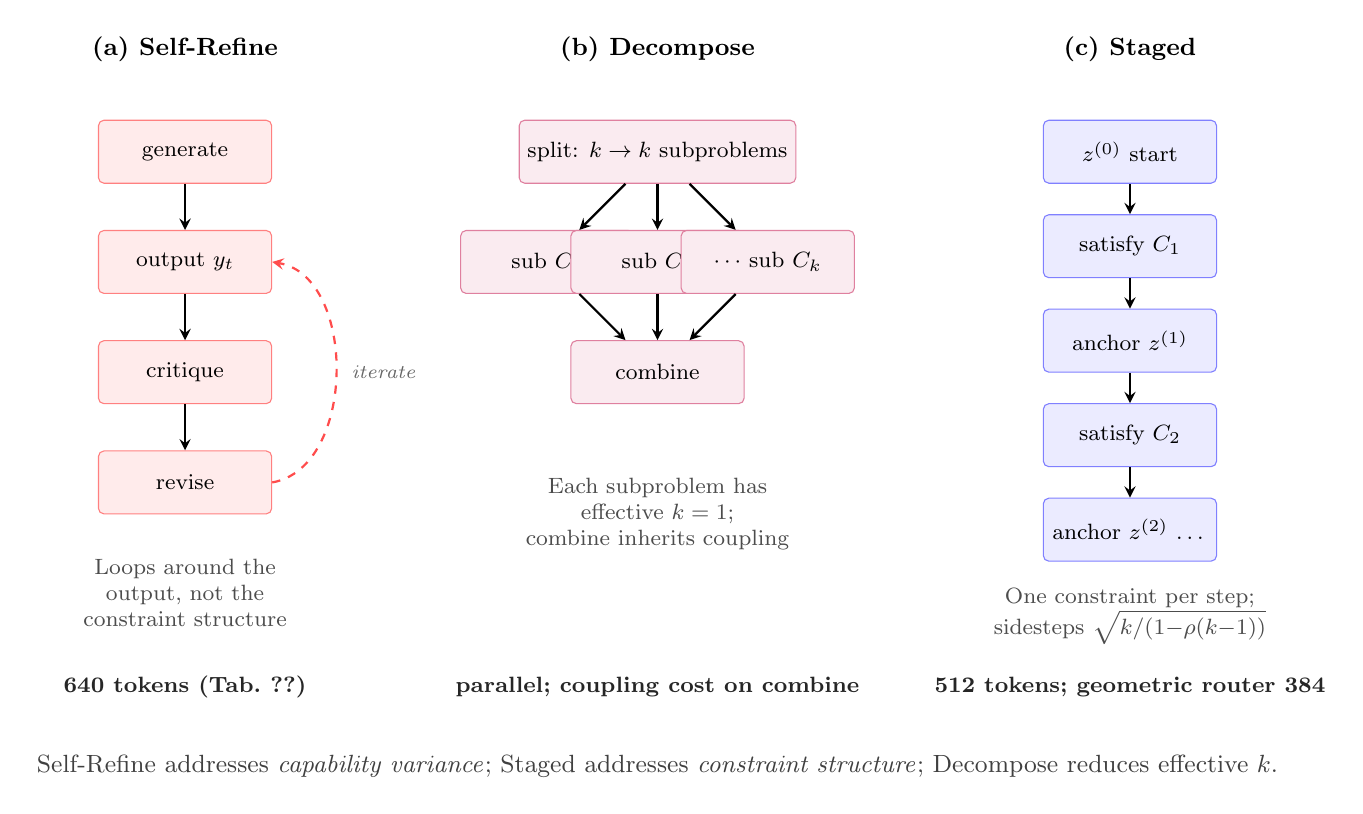
\begin{tikzpicture}[
    font=\normalsize,
    panel/.style={draw=black!30, rounded corners=3pt, inner sep=8pt},
    label/.style={font=\small\bfseries},
    sub/.style={font=\footnotesize, color=black!70},
    cost/.style={font=\footnotesize\bfseries, color=black!85},
    box/.style={draw, rounded corners=2pt, minimum height=8mm, minimum width=22mm, align=center, inner sep=3pt, fill=white, font=\footnotesize},
    refbox/.style={box, fill=red!8, draw=red!50},
    stagebox/.style={box, fill=blue!8, draw=blue!50},
    decombox/.style={box, fill=purple!8, draw=purple!50},
    anchor_node/.style={font=\scriptsize\itshape, color=black!60},
    arr/.style={->, thick, >=stealth},
    loop/.style={->, thick, >=stealth, dashed, color=red!70},
]
    % ============= Panel A: Self-Refine =============
    \node[label] (titleA) at (0, 4.5) {(a) Self-Refine};
    \node[refbox] (gen) at (0, 3.2) {generate};
    \node[refbox] (out) at (0, 1.8) {output $y_t$};
    \node[refbox] (crit) at (0, 0.4) {critique};
    \node[refbox] (rev) at (0, -1.0) {revise};
    \draw[arr] (gen) -- (out);
    \draw[arr] (out) -- (crit);
    \draw[arr] (crit) -- (rev);
    \draw[loop] (rev.east) to[bend right=80] node[anchor_node, right=2pt] {iterate} (out.east);
    \node[sub, align=center] at (0, -2.4) {Loops around the\\output, not the\\constraint structure};
    \node[cost] at (0, -3.6) {640 tokens (Tab.~\ref{tab:baselines})};

    % ============= Panel B: Decompose =============
    \node[label] (titleB) at (6.0, 4.5) {(b) Decompose};
    \node[decombox] (split) at (6.0, 3.2) {split: $k \to k$ subproblems};
    \node[decombox] (s1) at (4.6, 1.8) {sub $C_1$};
    \node[decombox] (s2) at (6.0, 1.8) {sub $C_2$};
    \node[decombox] (sk) at (7.4, 1.8) {$\cdots$ sub $C_k$};
    \node[decombox] (combine) at (6.0, 0.4) {combine};
    \draw[arr] (split) -- (s1);
    \draw[arr] (split) -- (s2);
    \draw[arr] (split) -- (sk);
    \draw[arr] (s1) -- (combine);
    \draw[arr] (s2) -- (combine);
    \draw[arr] (sk) -- (combine);
    \node[sub, align=center] at (6.0, -1.4) {Each subproblem has\\effective $k=1$;\\combine inherits coupling};
    \node[cost] at (6.0, -3.6) {parallel; coupling cost on combine};

    % ============= Panel C: Staged =============
    \node[label] (titleC) at (12.0, 4.5) {(c) Staged};
    \node[stagebox] (z0) at (12.0, 3.2) {$z^{(0)}$ start};
    \node[stagebox] (s1c) at (12.0, 2.0) {satisfy $C_1$};
    \node[stagebox] (a1) at (12.0, 0.8) {anchor $z^{(1)}$};
    \node[stagebox] (s2c) at (12.0, -0.4) {satisfy $C_2$};
    \node[stagebox] (a2) at (12.0, -1.6) {anchor $z^{(2)}$ \dots};
    \draw[arr] (z0) -- (s1c);
    \draw[arr] (s1c) -- (a1);
    \draw[arr] (a1) -- (s2c);
    \draw[arr] (s2c) -- (a2);
    \node[sub, align=center] at (12.0, -2.7) {One constraint per step;\\sidesteps $\sqrt{k/(1{-}\rho(k{-}1))}$};
    \node[cost] at (12.0, -3.6) {512 tokens; geometric router 384};

    % Bottom summary line
    \node[font=\small, color=black!75, align=center] at (6.0, -4.6) {%
        Self-Refine addresses \emph{capability variance}; Staged addresses \emph{constraint structure}; Decompose reduces effective $k$.%
    };
\end{tikzpicture}
}
\caption{Three control protocols on the same multi-constraint problem (schematic). Self-refine cycles around the output token sequence and addresses capability variance; it does not directly navigate constraint geometry. Decompose splits $k$ constraints into sub-problems with effective $k{=}1$, paying coupling cost at the combine step. Staged satisfies one constraint per step, anchoring intermediate states; this sidesteps the diagonal cost penalty $\sqrt{k/(1-\rho(k-1))}$. Token counts from Table~\ref{tab:baselines}. Provenance: \texttt{ci/illustration\_lineage.json}; image draft via gpt-5.4-image-2 used for visual exploration only (the draft model interpreted the source block more narrowly than the comparison the body argues; the deterministic redraw widens to the three-protocol contrast). Schematic illustration only; not empirical evidence.}
\label{fig:staging_vs_refine}
\end{figure}
